\documentclass[10pt]{article}
\usepackage[margin=1in]{geometry} 
\usepackage{enumerate, xfrac, color, graphicx}
\usepackage{amsmath,amsthm,amssymb,amsfonts,mathabx}
\usepackage{booktabs}
\usepackage{caption}
\usepackage{algorithm}
\usepackage{algpseudocode}
\usepackage{pifont}
\usepackage{listings, courier}
\graphicspath{{/Users/mfzhao/Dropbox/}}
\newcommand{\N}{\mathbb{N}}
\newcommand{\Z}{\mathbb{Z}}
\lstset{breaklines=true, basicstyle=\small\ttfamily, language=R, backgroundcolor=\color{highlight}, stepnumber=5}

\definecolor{highlight}{RGB}{248,248,248}

\begin{document}
	\title{6.867 Problem Set 2}
	\maketitle


\subsubsection*{Logistic Regression}

\begin{table}
\captionof{table}{Performance of Logistic Regression on provided data sets with a decision boundary of 0.5}
\begin{tabular}{llllll}
\toprule
{} & dataset & classification error (training set) & classification error (validation set) \\
\midrule
  & data\_stdev1 & 0.00\% & 0.00\% \\
  & data\_stdev2 & 9.25\% & 8.00\% \\
  & data\_stdev4 & 26.00\% & 24.75\% \\
  & data\_nonsep & 48.50\% & 50.75\% \\
\bottomrule
\end{tabular}
\end{table}


\begin{figure}[ht]
	\centering
	\begin{minipage}[b]{.24\linewidth}
		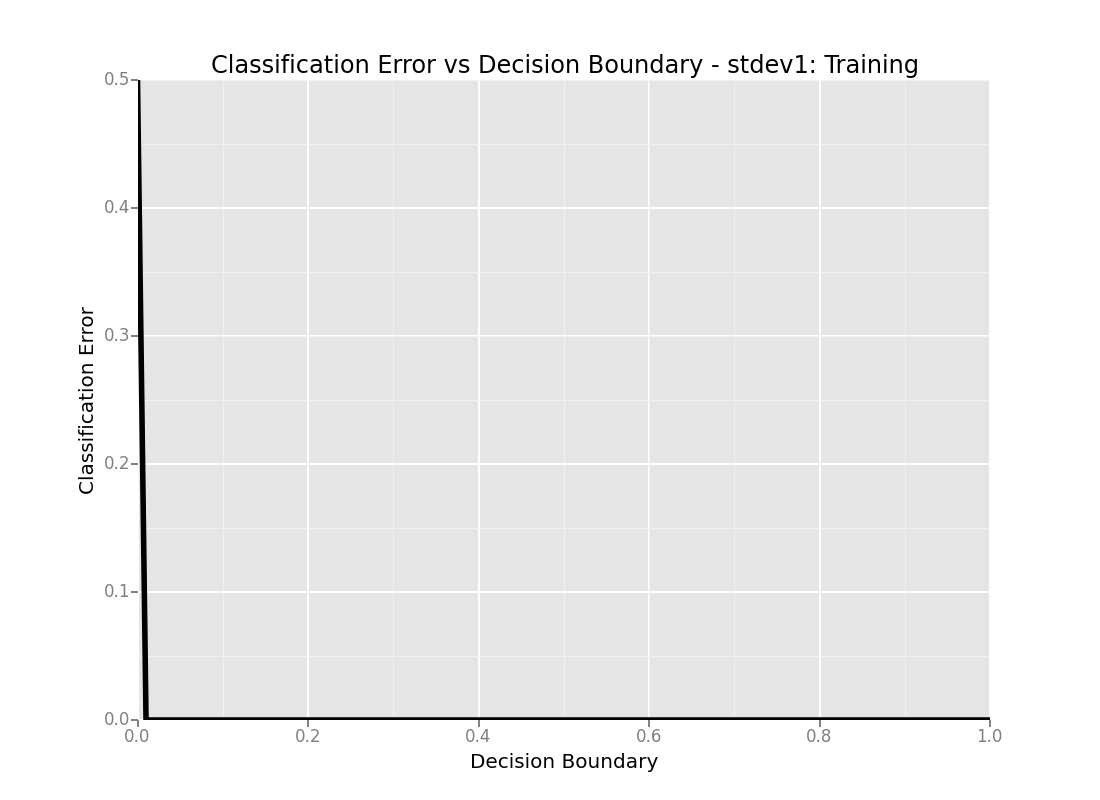
\includegraphics[width=1\linewidth, height=1in]{CEDB_stdev1_train.png}
		\caption*{stdev1 (Training)}
	\end{minipage}
	\begin{minipage}[b]{.24\linewidth}
		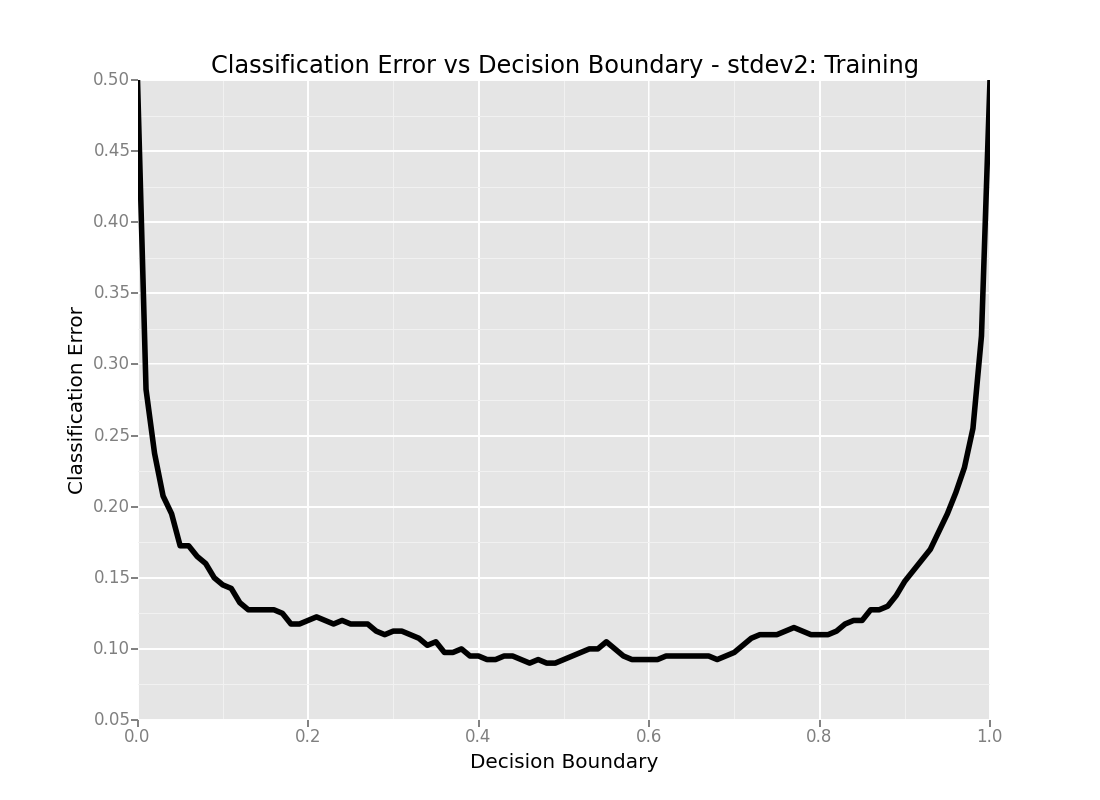
\includegraphics[width=1\linewidth, height=1in]{CEDB_stdev2_train.png}
		\caption*{stdev2 (Training)}
	\end{minipage}
	\begin{minipage}[b]{.24\linewidth}
		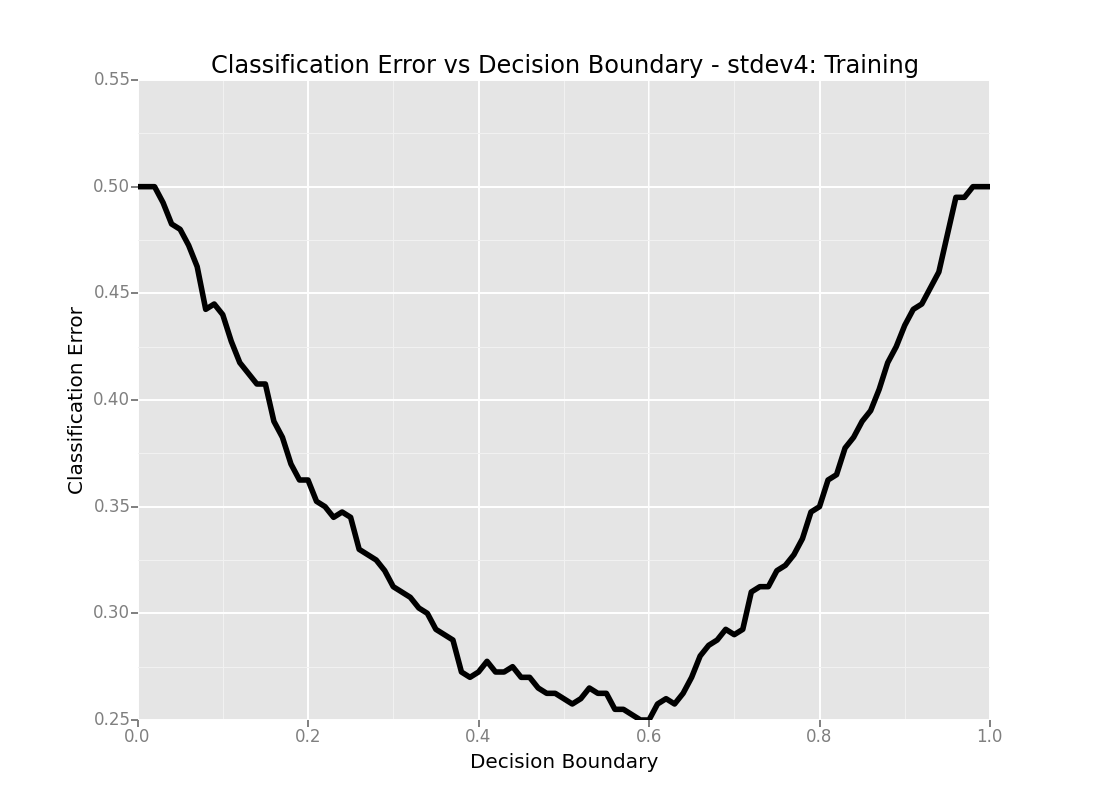
\includegraphics[width=1\linewidth, height=1in]{CEDB_stdev4_train.png}
		\caption*{stdev4 (Training)}
	\end{minipage}
	\begin{minipage}[b]{.24\linewidth}
		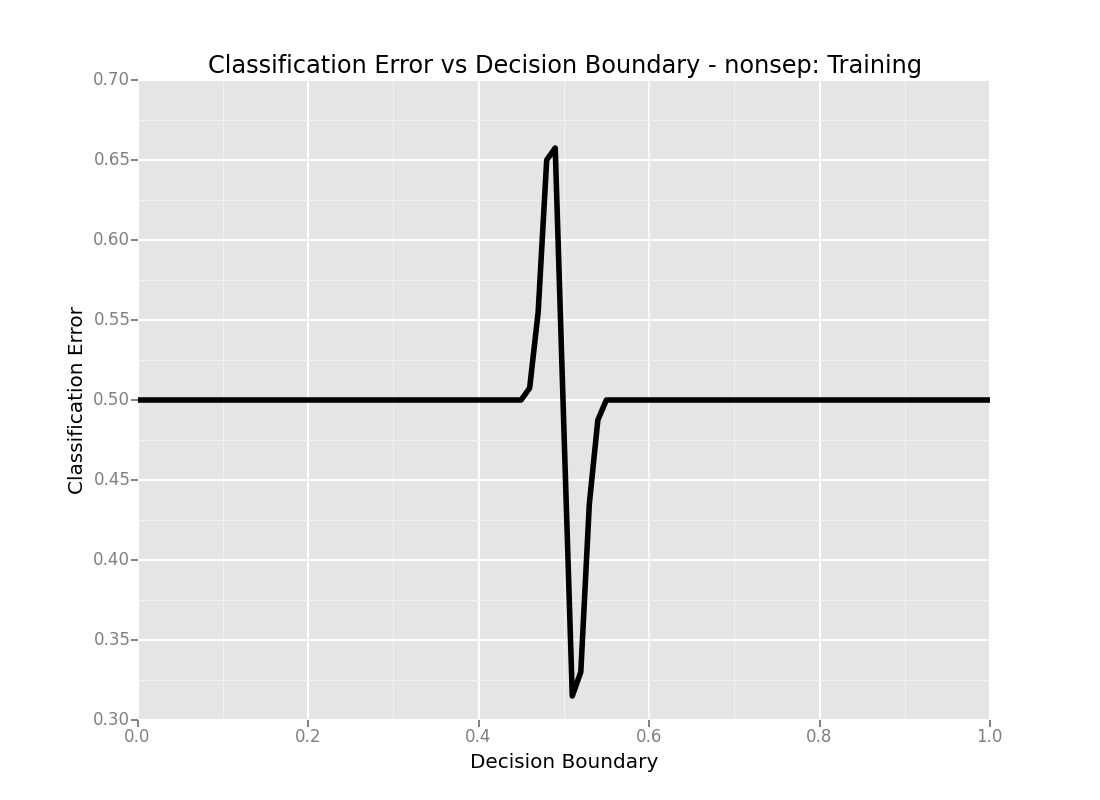
\includegraphics[width=1\linewidth, height=1in]{CEDB_nonsep_train.png}
		\caption*{nonsep (Training)}
	\end{minipage}
		\begin{minipage}[b]{.24\linewidth}
		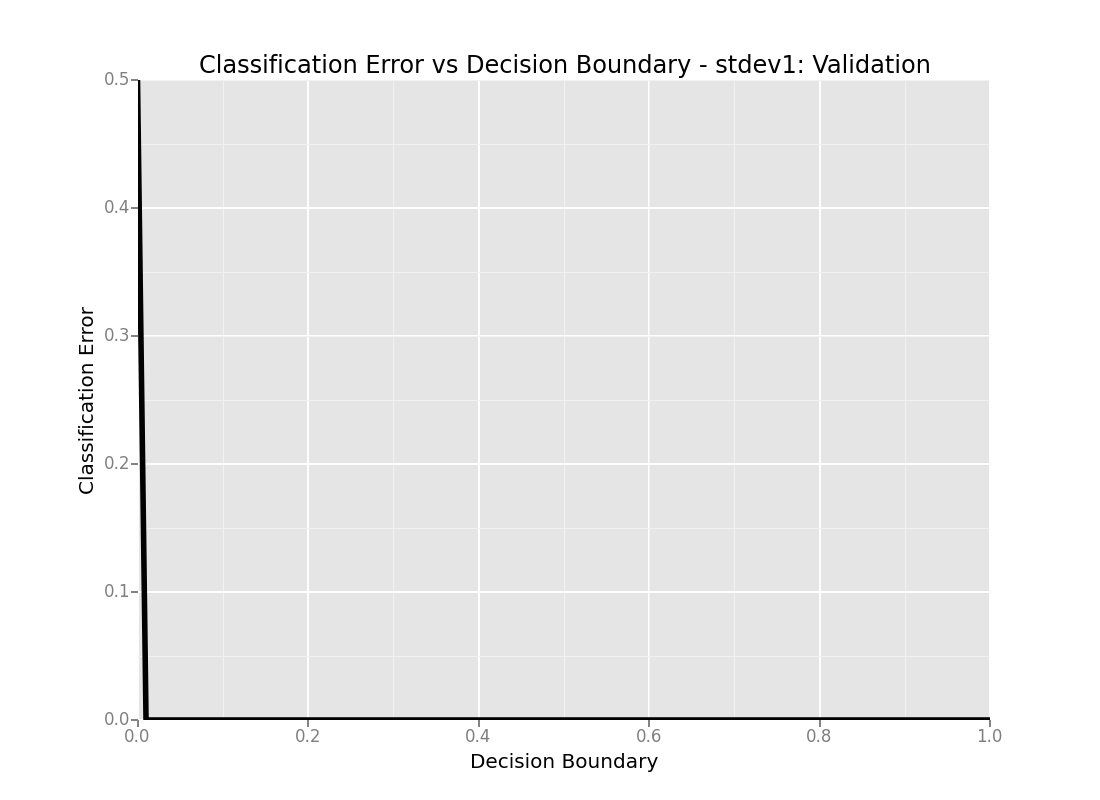
\includegraphics[width=1\linewidth, height=1in]{CEDB_stdev1_validation.png}
		\caption*{stdev1 (Validation)}
	\end{minipage}
	\begin{minipage}[b]{.24\linewidth}
		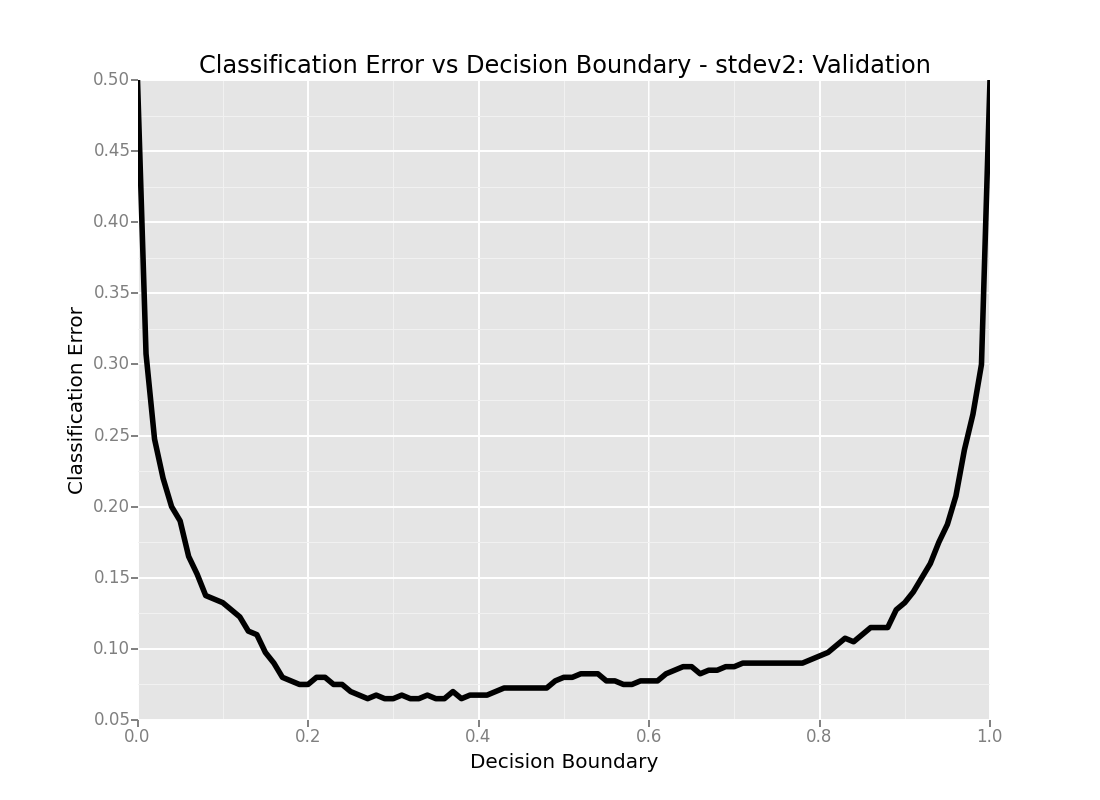
\includegraphics[width=1\linewidth, height=1in]{CEDB_stdev2_validation.png}
		\caption*{stdev2 (Validation)}
	\end{minipage}
	\begin{minipage}[b]{.24\linewidth}
		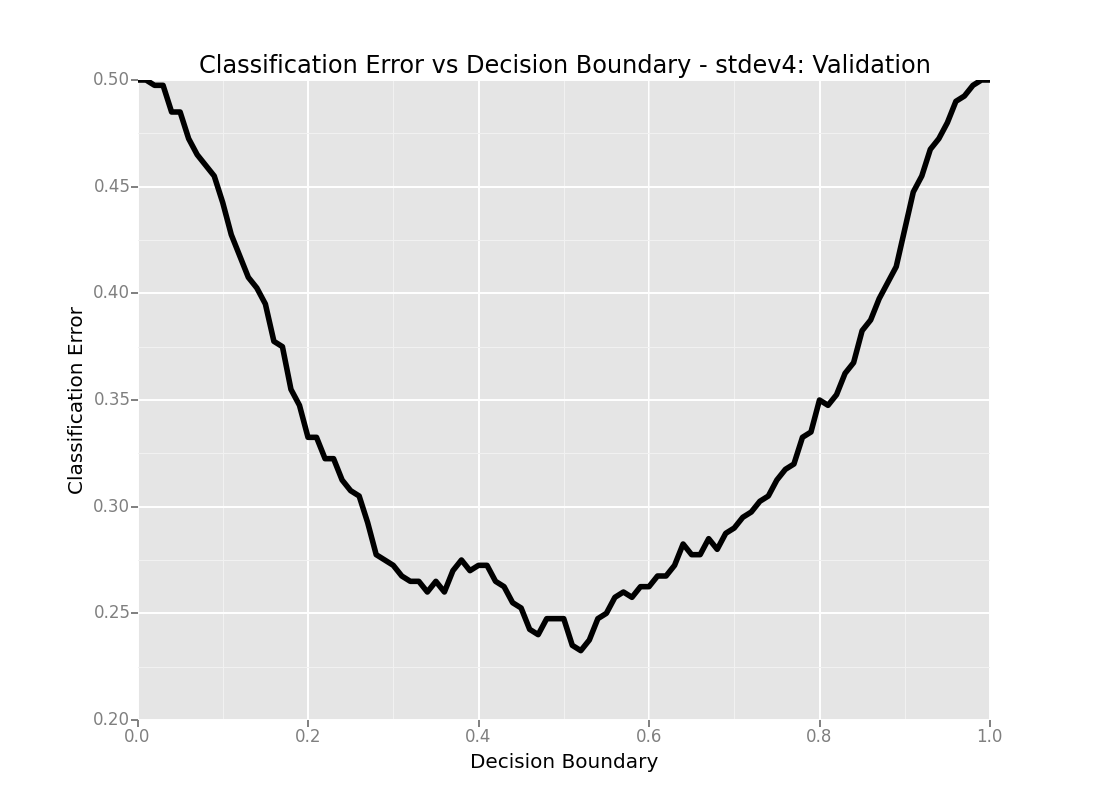
\includegraphics[width=1\linewidth, height=1in]{CEDB_stdev4_validation.png}
		\caption*{stdev4 (Validation)}
	\end{minipage}
	\begin{minipage}[b]{.24\linewidth}
		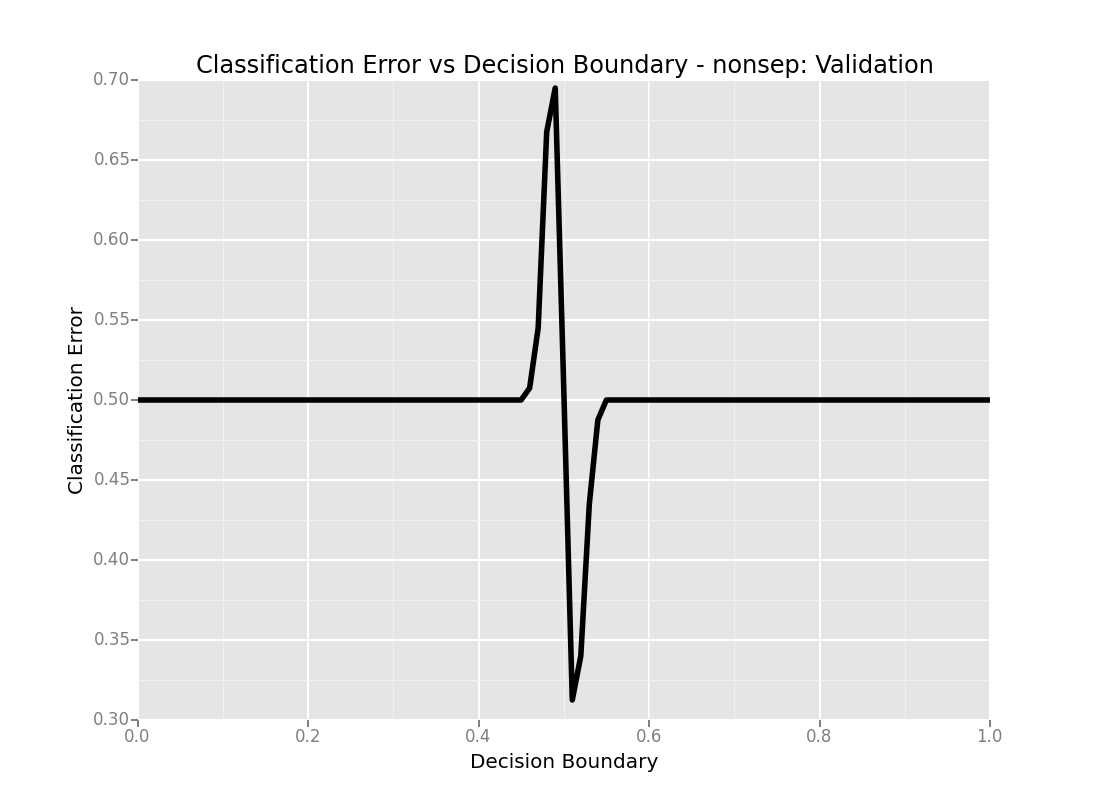
\includegraphics[width=1\linewidth, height=1in]{CEDB_nonsep_validation.png}
		\caption*{nonsep (Validation)}
	\end{minipage}
	\caption{The classification error of Logistic Regression as a function of our choice of a decision boundary for the stdev1, stdev2, stdev4, and nonsep (training and validation) datasets}
\end{figure}


\begin{figure}[ht]
	\centering
	\begin{minipage}[b]{.24\linewidth}
		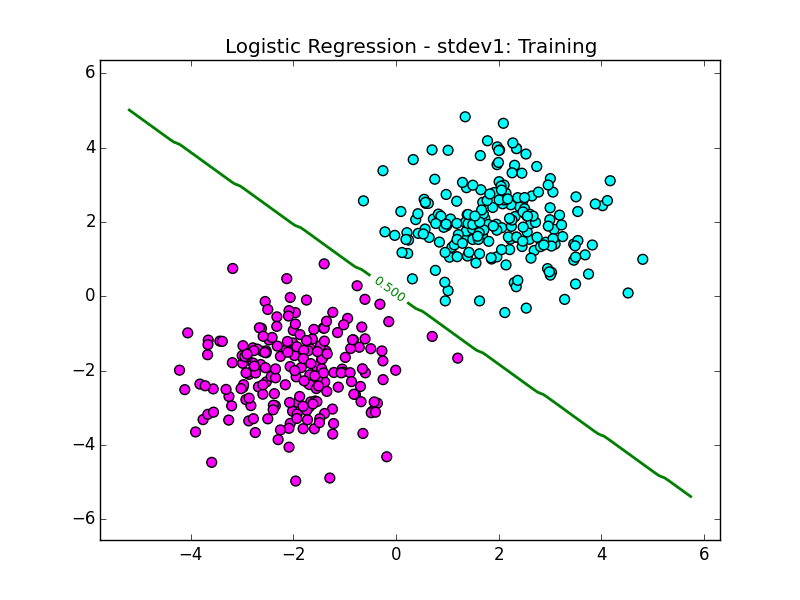
\includegraphics[width=1\linewidth, height=1in]{LR_stdev1_train.png}
		\caption*{stdev1 (Training)}
	\end{minipage}
	\begin{minipage}[b]{.24\linewidth}
		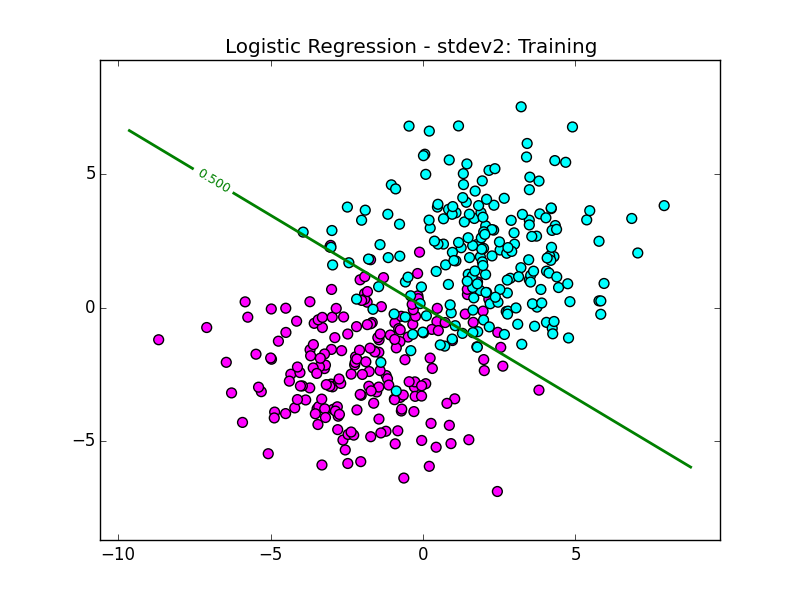
\includegraphics[width=1\linewidth, height=1in]{LR_stdev2_train.png}
		\caption*{stdev2 (Training)}
	\end{minipage}
	\begin{minipage}[b]{.24\linewidth}
		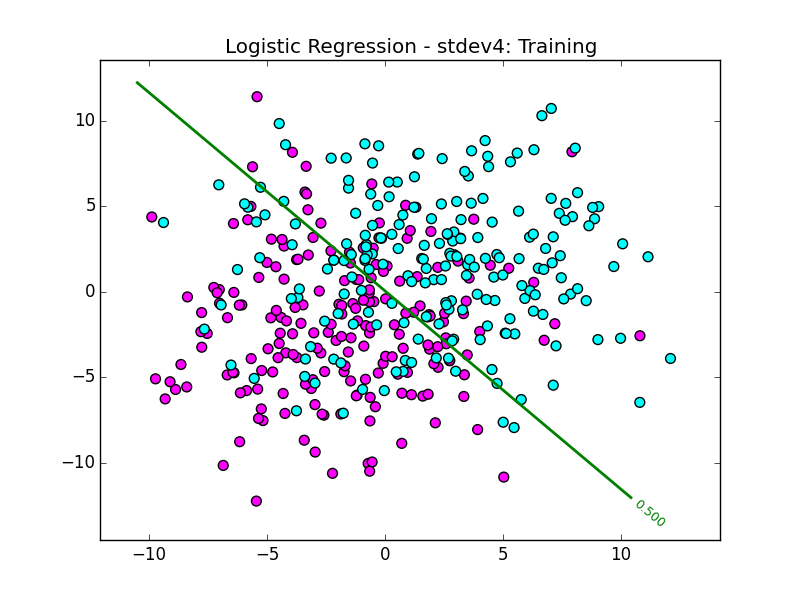
\includegraphics[width=1\linewidth, height=1in]{LR_stdev4_train.png}
		\caption*{stdev4 (Training)}
	\end{minipage}
	\begin{minipage}[b]{.24\linewidth}
		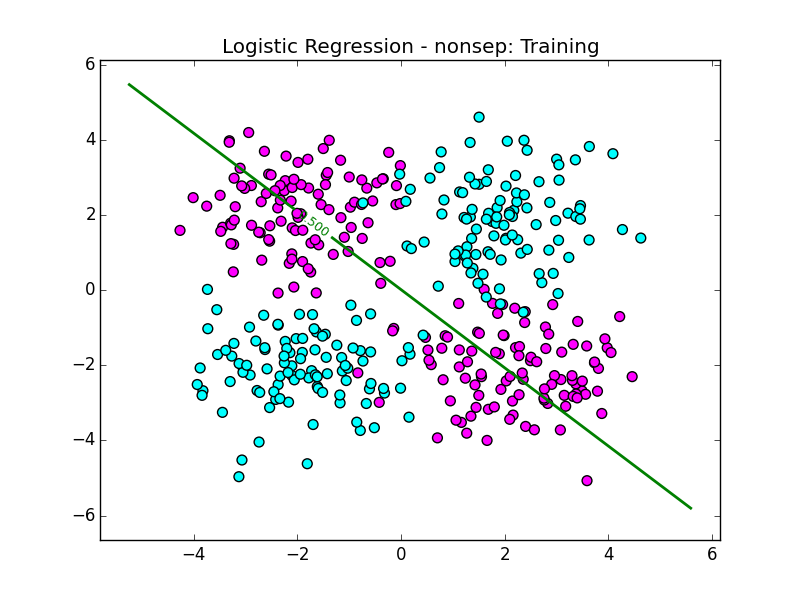
\includegraphics[width=1\linewidth, height=1in]{LR_nonsep_train.png}
		\caption*{nonsep (Training)}
	\end{minipage}
		\begin{minipage}[b]{.24\linewidth}
		\includegraphics[width=1\linewidth, height=1in]{LR_stdev1_validation.png}
		\caption*{stdev1 (Validation)}
	\end{minipage}
	\begin{minipage}[b]{.24\linewidth}
		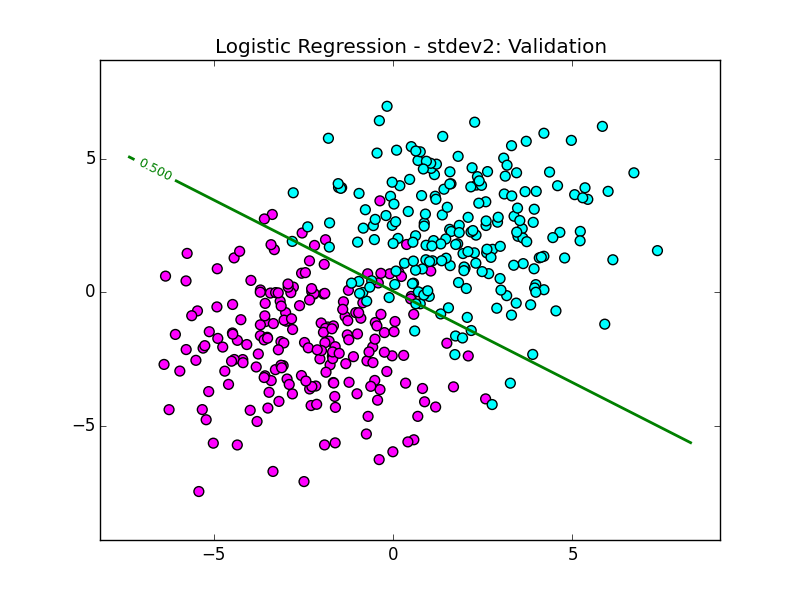
\includegraphics[width=1\linewidth, height=1in]{LR_stdev2_validation.png}
		\caption*{stdev2 (Validation)}
	\end{minipage}
	\begin{minipage}[b]{.24\linewidth}
		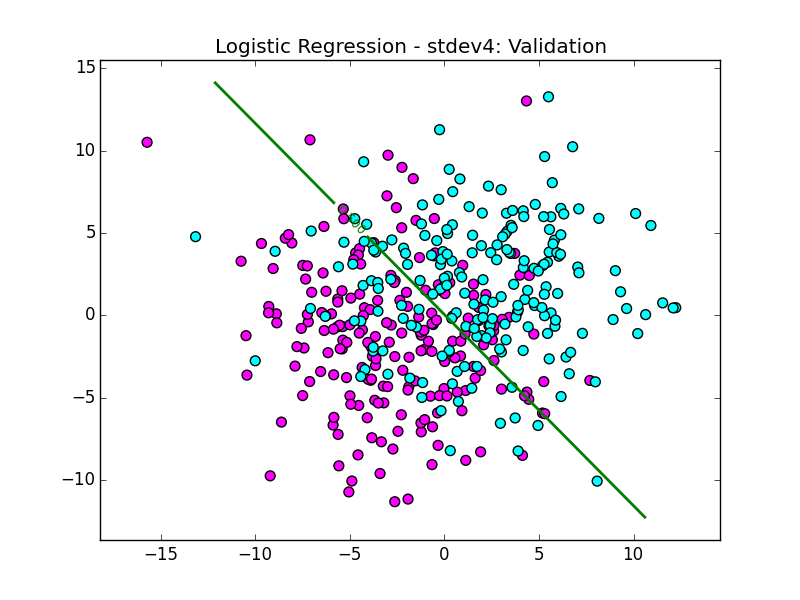
\includegraphics[width=1\linewidth, height=1in]{LR_stdev4_validation.png}
		\caption*{stdev4 (Validation)}
	\end{minipage}
	\begin{minipage}[b]{.24\linewidth}
		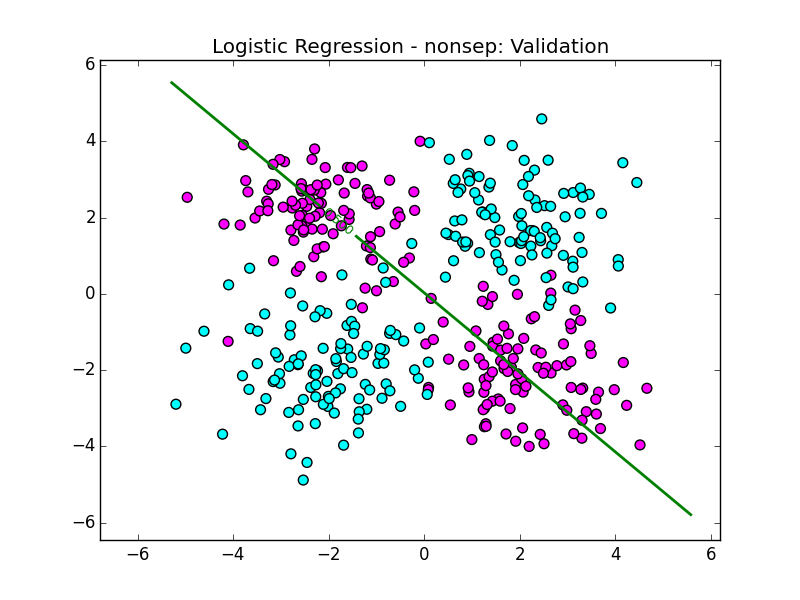
\includegraphics[width=1\linewidth, height=1in]{LR_nonsep_validation.png}
		\caption*{nonsep (Validation)}
	\end{minipage}
	\caption{The decision boundaries generated by Logistic Regression plotted against the stdev1, stdev2, stdev4, and nonsep (training and validation) datasets}
\end{figure}

\begin{figure}[ht]
	\centering
	\begin{minipage}[b]{.24\linewidth}
		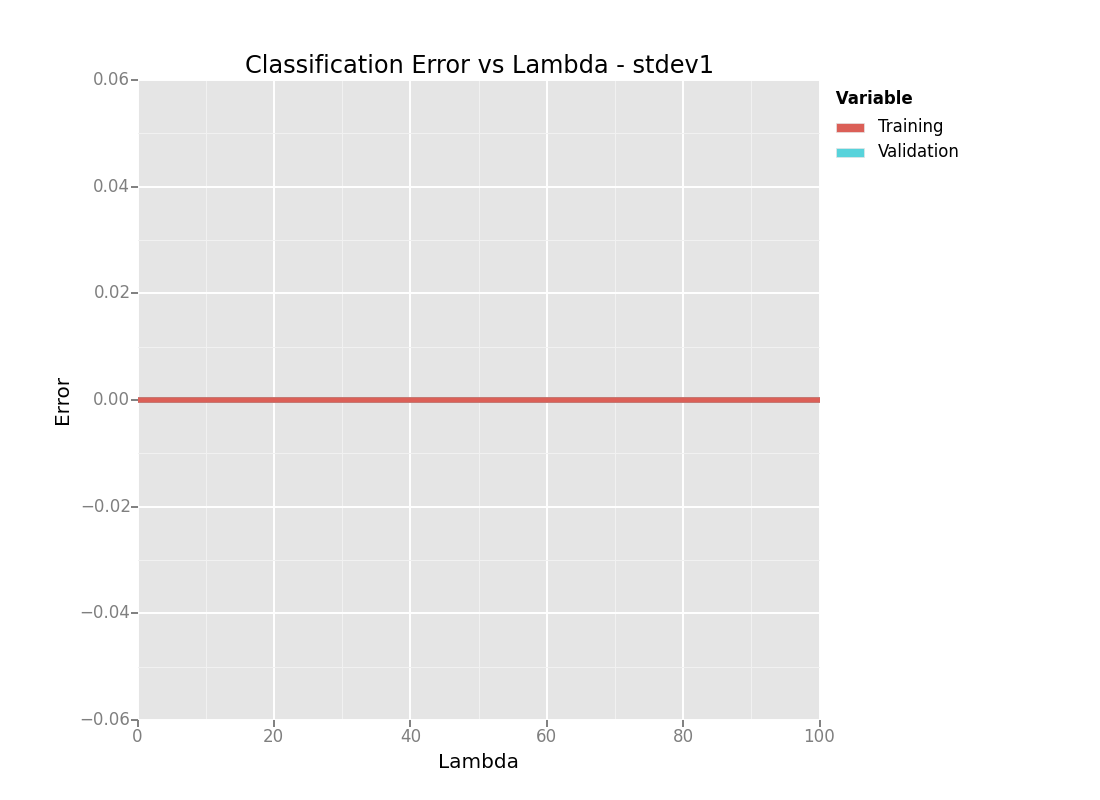
\includegraphics[width=1\linewidth, height=1in]{CErr_lambda_stdev1.png}
		\caption*{Classification Error - stdev1}
	\end{minipage}
	\begin{minipage}[b]{.24\linewidth}
		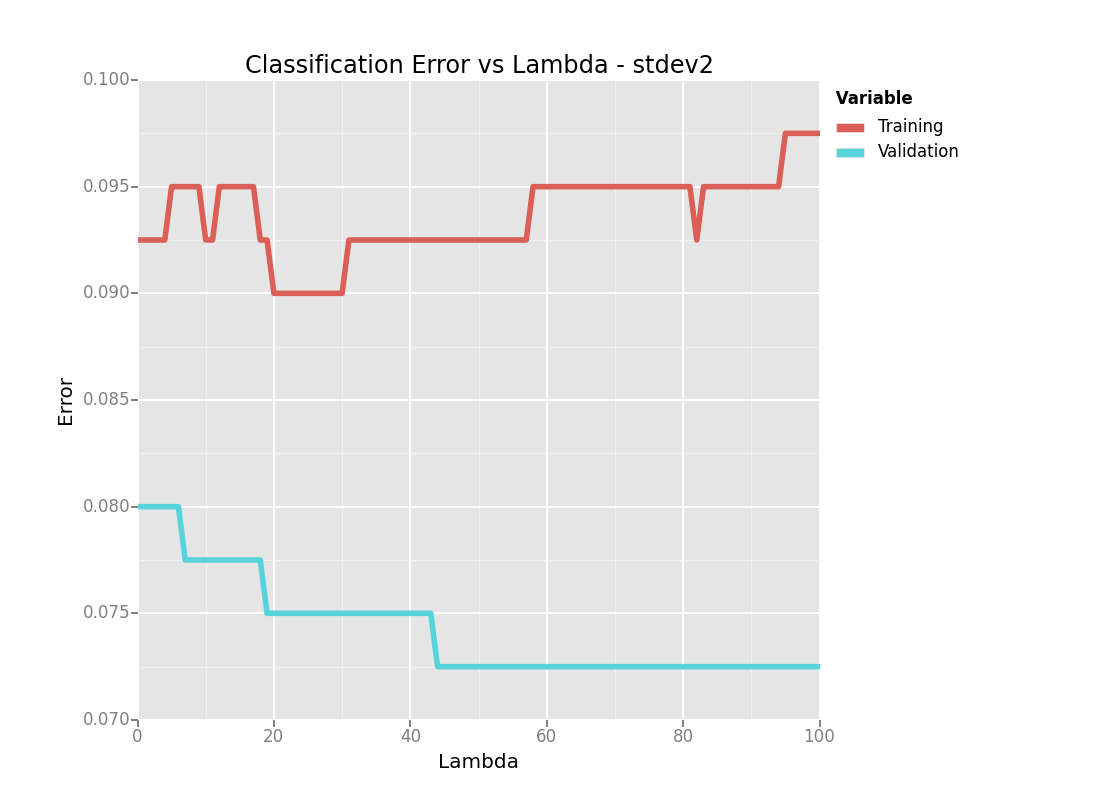
\includegraphics[width=1\linewidth, height=1in]{CErr_lambda_stdev2.png}
		\caption*{Classification Error - stdev2}
	\end{minipage}
	\begin{minipage}[b]{.24\linewidth}
		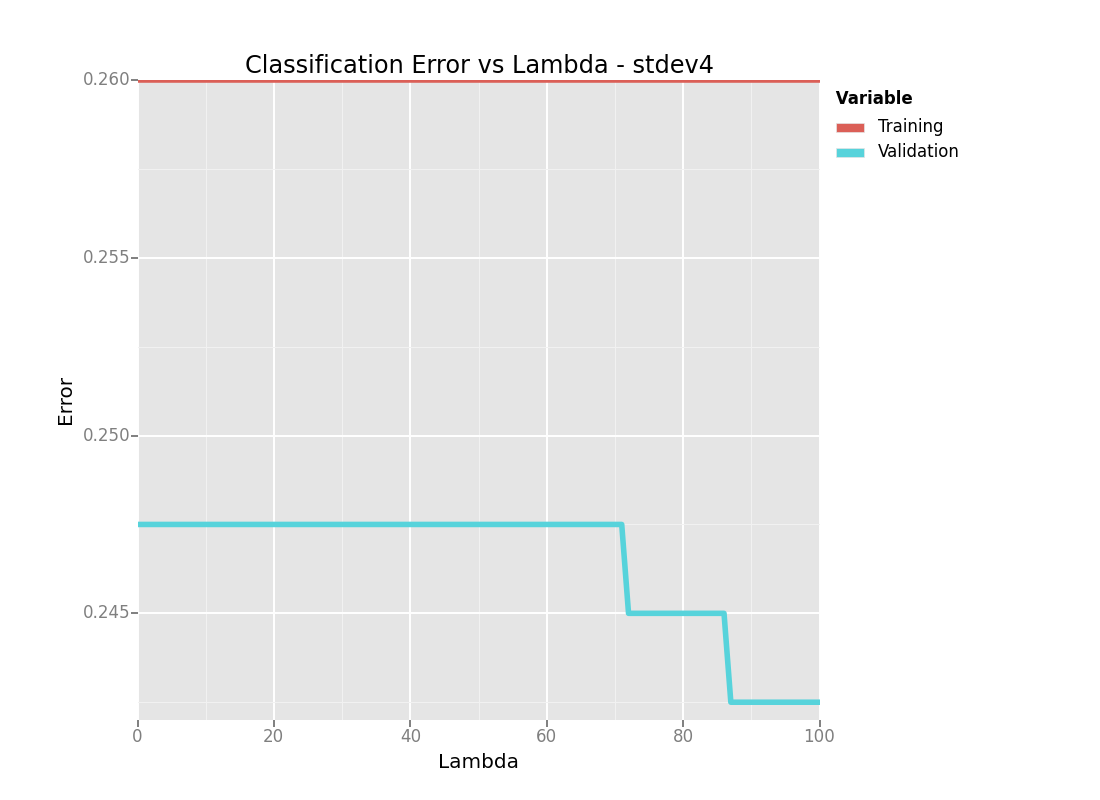
\includegraphics[width=1\linewidth, height=1in]{CErr_lambda_stdev4.png}
		\caption*{Classification Error - stdev4}
	\end{minipage}
	\begin{minipage}[b]{.24\linewidth}
		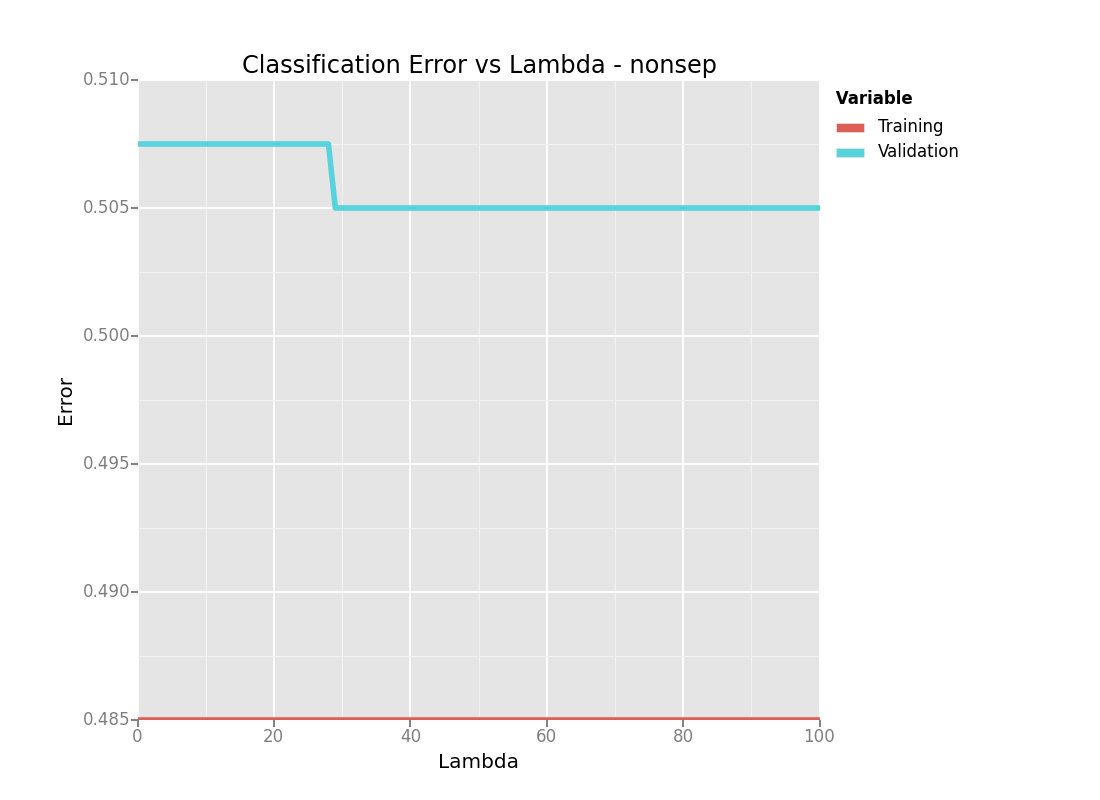
\includegraphics[width=1\linewidth, height=1in]{CErr_lambda_nonsep.png}
		\caption*{Classification Error - nonsep}
	\end{minipage}
		\begin{minipage}[b]{.24\linewidth}
		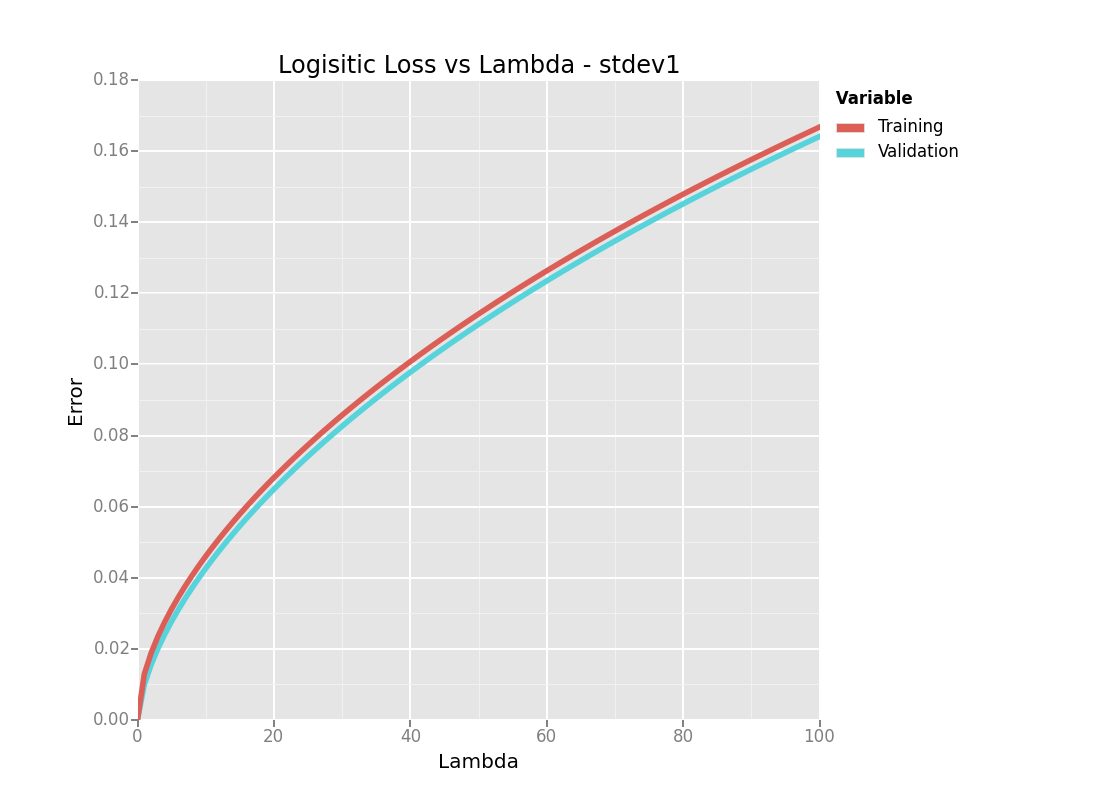
\includegraphics[width=1\linewidth, height=1in]{Loss_lambda_stdev1.png}
		\caption*{Logistic Loss - stdev1}
	\end{minipage}
	\begin{minipage}[b]{.24\linewidth}
		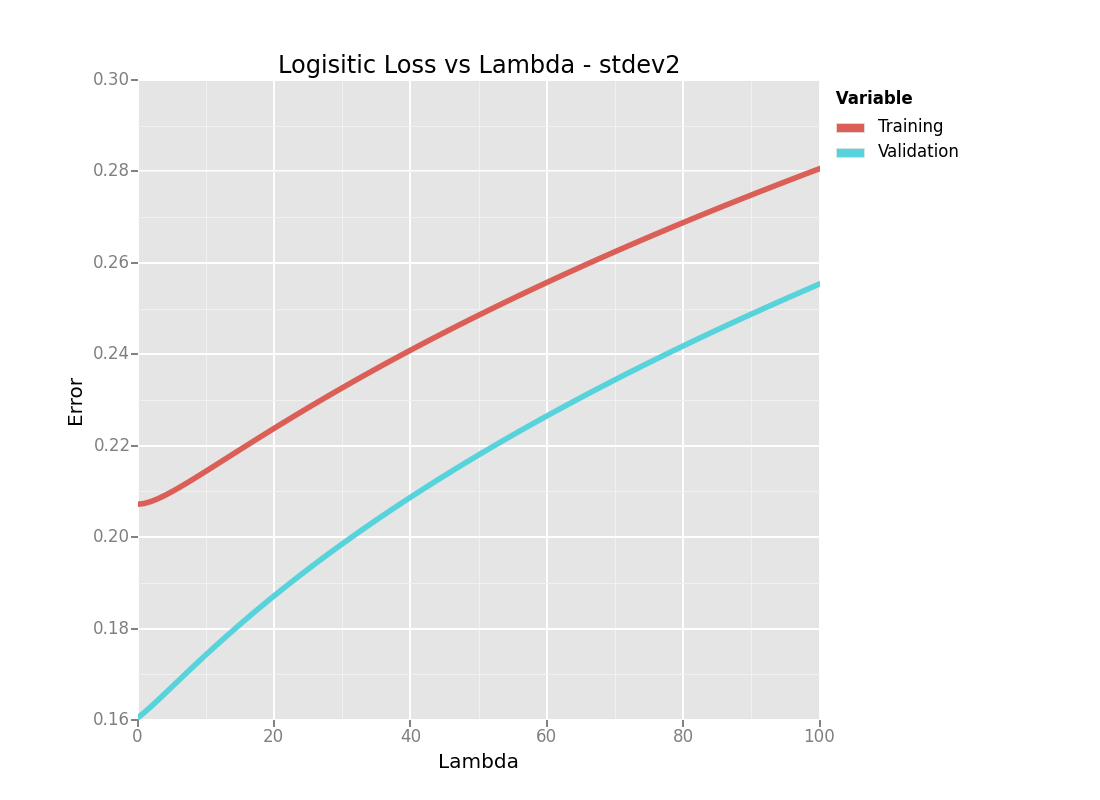
\includegraphics[width=1\linewidth, height=1in]{Loss_lambda_stdev2.png}
		\caption*{Logistic Loss - stdev2}
	\end{minipage}
	\begin{minipage}[b]{.24\linewidth}
		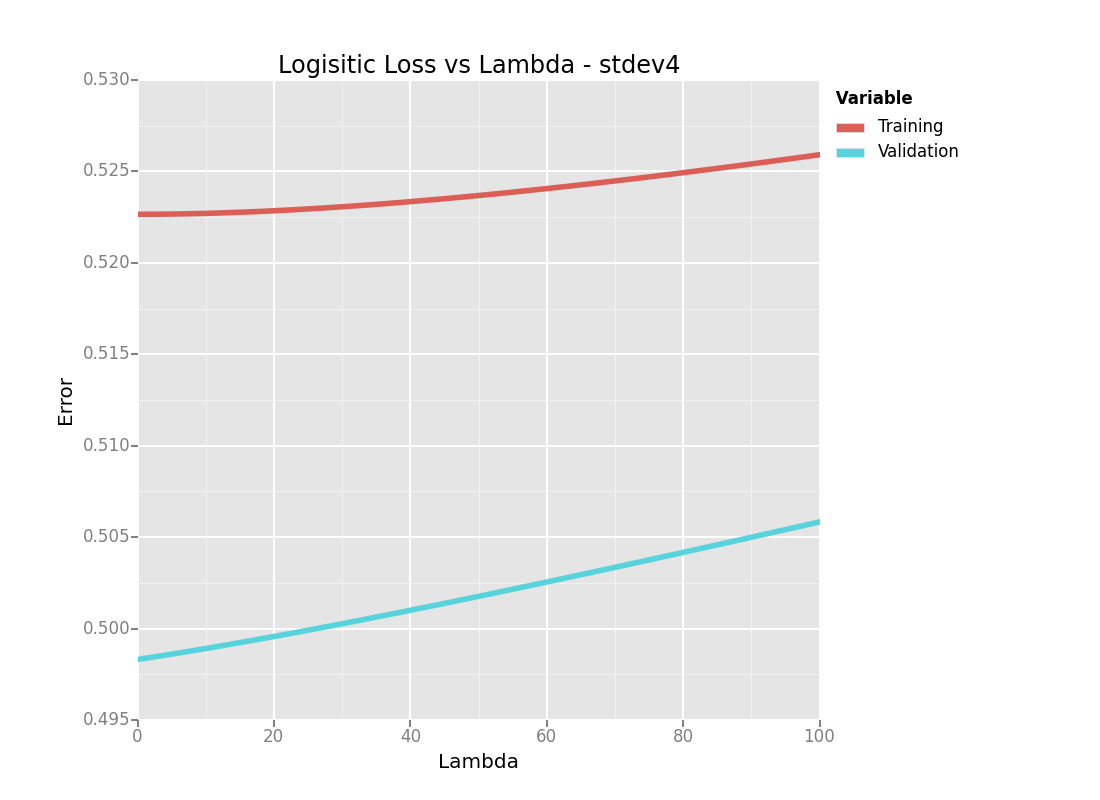
\includegraphics[width=1\linewidth, height=1in]{Loss_lambda_stdev4.png}
		\caption*{Logistic Loss - stdev4}
	\end{minipage}
	\begin{minipage}[b]{.24\linewidth}
		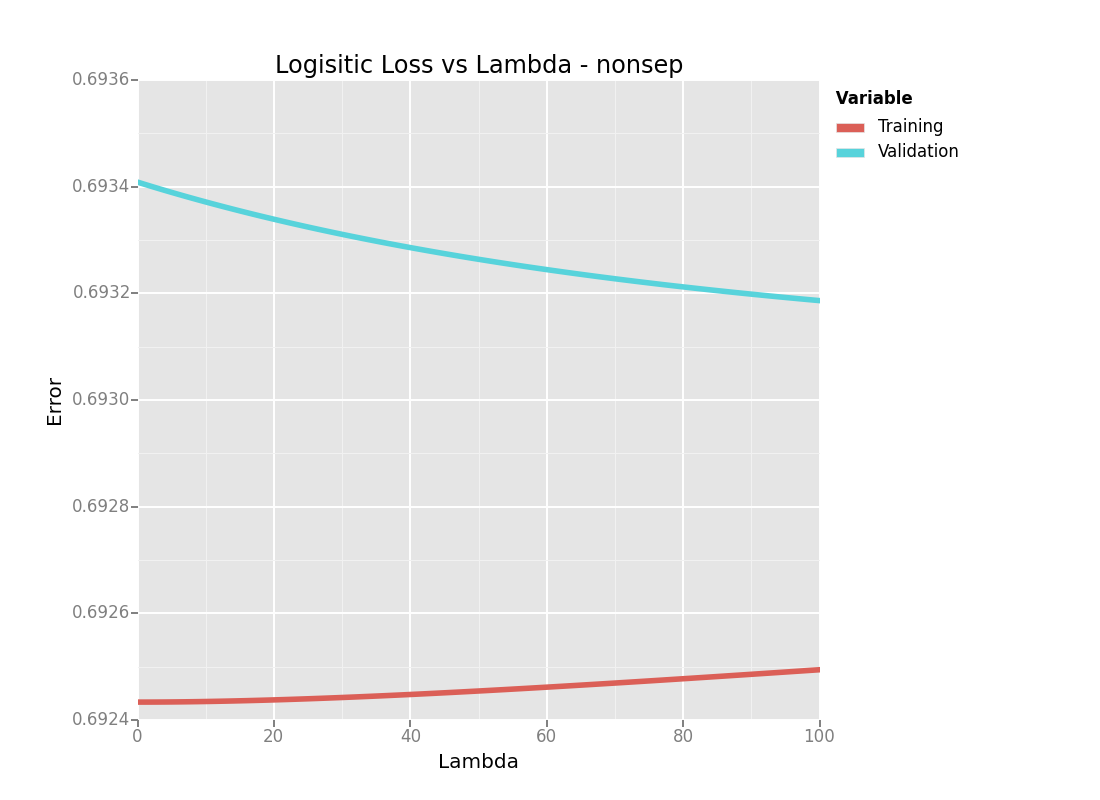
\includegraphics[width=1\linewidth, height=1in]{Loss_lambda_nonsep.png}
		\caption*{Logistic Loss - nonsep}
	\end{minipage}
	\caption{Classification Error (for a decision boundary of 0.5) and Logistic Loss of Logistic Regression as a function of the L2 penalty $\lambda$}
\end{figure}


\subsubsection*{Support Vector Machines}

Let's now compare the performance of SVM to that of logistic regression for classification problems. To illustrate the objective and constraints of the support vector machine, we have included below the explicit objective we would optimize over, as well as the constraints, for the dual form of a linear SVM with slack variables. The equations below correspond to the 2D problem where we have positive examples (1, 2), (2, 2) and negative examples (0, 0), (-2, 3).

\[
\min_{\alpha_1, \alpha_2, \alpha_3, \alpha_4}
\frac{1}{2}
\begin{bmatrix}
    \alpha_1 & \alpha_2 & \alpha_3 & \alpha_4 \\
\end{bmatrix}
\begin{bmatrix}
    5       & 6 & 0 & -4 \\
    6       & 8 & 0 & -2 \\
    0       & 0 & 0 & 0 \\
    -4       & -2 & 0 & 13 \\
\end{bmatrix}
\begin{bmatrix}
    \alpha_1 \\
    \alpha_2 \\
    \alpha_3 \\
    \alpha_4 \\
\end{bmatrix} 
+
\begin{bmatrix}
    -1       & -1 & -1 & -1 \\
\end{bmatrix}
\begin{bmatrix}
    \alpha_1 \\
    \alpha_2 \\
    \alpha_3 \\
    \alpha_4 \\
\end{bmatrix} 
\]

\begin{center}
s.t.
\end{center}

\[
\begin{bmatrix}
    -1 & 0 & 0 & 0 \\
    0 & -1 & 0 & 0 \\
    0 & 0 & -1 & 0 \\
    0 & 0 & 0 & -1 \\
    1 & 0 & 0 &0 \\
    0 & 1 & 0 & 0 \\
    0 & 0 & 1 & 0 \\
    0 & 0 & 0 & 1 \\
\end{bmatrix}
\begin{bmatrix}
    \alpha_1 \\
    \alpha_2 \\
    \alpha_3 \\
    \alpha_4 \\
\end{bmatrix} 
\leq
\begin{bmatrix}
0 \\
0 \\ 
0 \\ 
0 \\ 
C \\
C \\ 
C \\ 
C \\
\end{bmatrix},
\]

\[
\begin{bmatrix}
    1 & 1 & -1 & -1 \\
\end{bmatrix}
\begin{bmatrix}
    \alpha_1 \\
    \alpha_2 \\
    \alpha_3 \\
    \alpha_4 \\
\end{bmatrix} 
= 0
\]

\begin{table}
\captionof{table}{Performance of Linear SVM on provided data sets}
\begin{tabular}{c c|c|c|c|c|c}
\toprule
{} & dataset & $w_0$ & $w_1$ & $w_2$ & classification error rate (training) & classification error rate (validation) \\
\midrule
  & data\_stdev1 & 0.31 & 5.42 & 0.87 & 0.00\% & 0.00\% \\
  & data\_stdev2 & 9.09e-2 & 9.83e1 & 9.11e1 & 9.50\% & 7.50\% \\
  & data\_stdev4 & -2.05e-2 & 2.58e2 & 2.40e2 & 26.00\% & 23.50\% \\
  & data\_nonsep & 2.56e-3 & 4.23e2 & 3.84e2 & 49.50\% & 51.25\% \\
\bottomrule
\end{tabular}
\end{table}

\begin{figure}[ht]
	\centering
	\begin{minipage}[b]{.24\linewidth}
		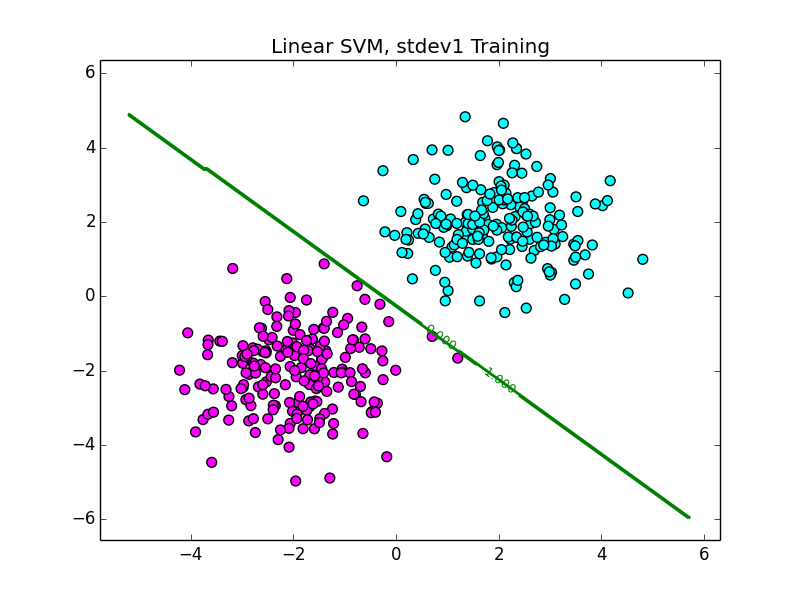
\includegraphics[width=1\linewidth, height=1in]{linear_svm_stdev1_train.png}
		\caption*{stdev1 (Training)}
	\end{minipage}
	\begin{minipage}[b]{.24\linewidth}
		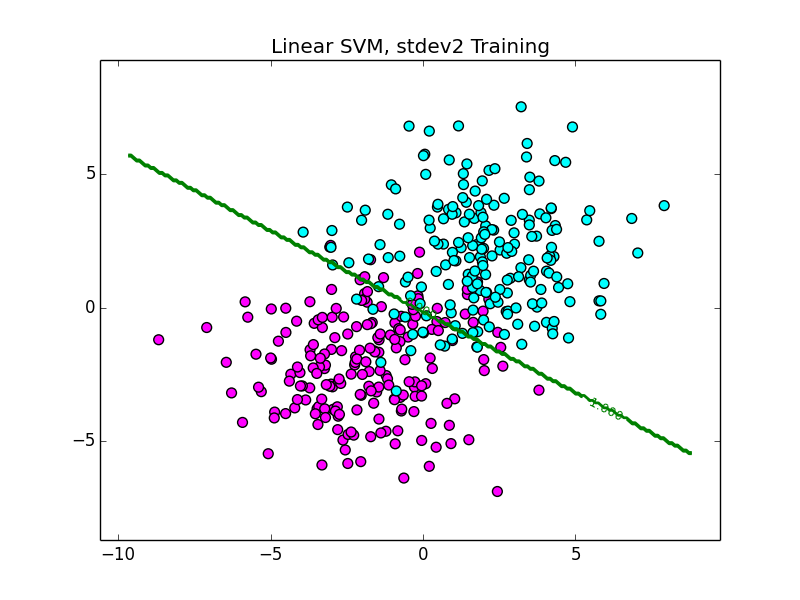
\includegraphics[width=1\linewidth, height=1in]{linear_svm_stdev2_train.png}
		\caption*{stdev2 (Training)}
	\end{minipage}
	\begin{minipage}[b]{.24\linewidth}
		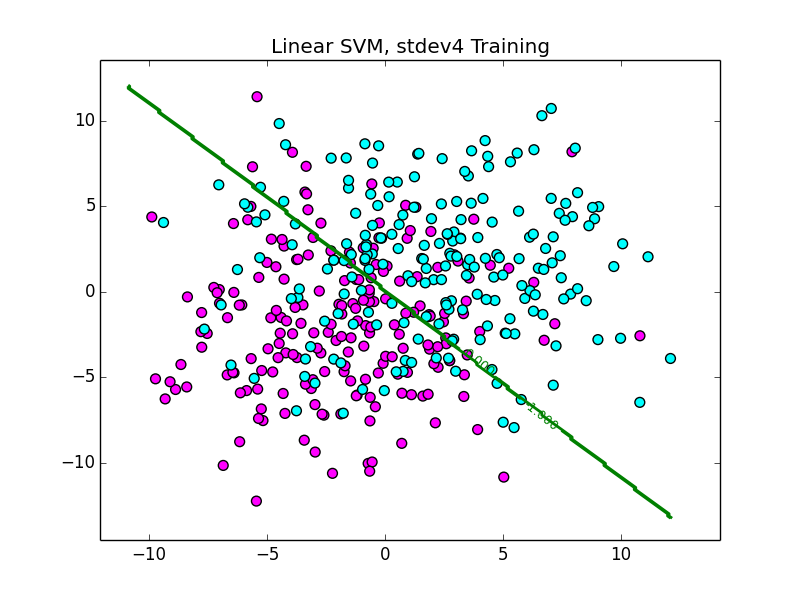
\includegraphics[width=1\linewidth, height=1in]{linear_svm_stdev4_train.png}
		\caption*{stdev4 (Training)}
	\end{minipage}
	\begin{minipage}[b]{.24\linewidth}
		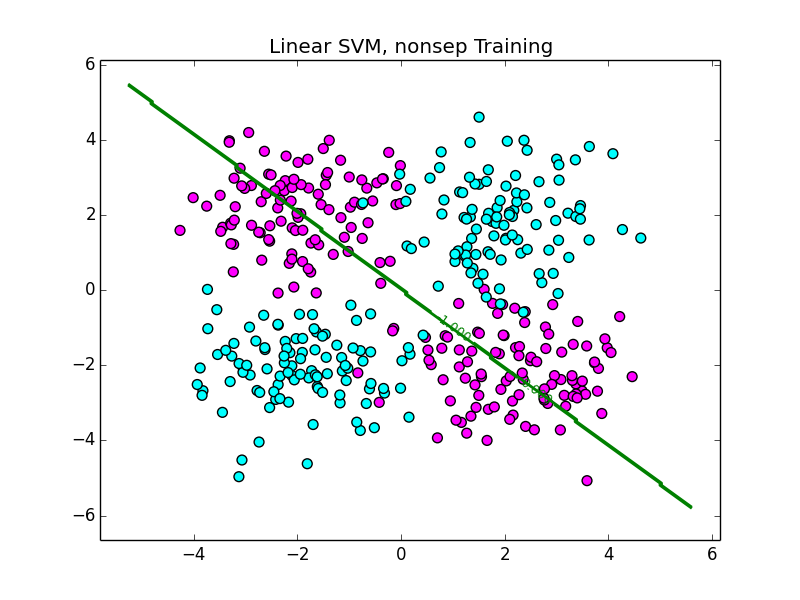
\includegraphics[width=1\linewidth, height=1in]{linear_svm_nonsep_train.png}
		\caption*{nonsep (Training)}
	\end{minipage}
		\begin{minipage}[b]{.24\linewidth}
		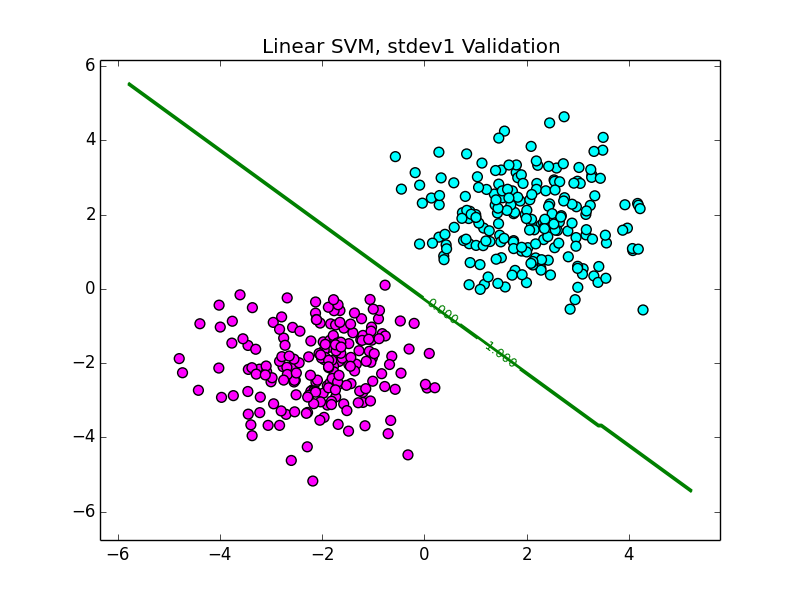
\includegraphics[width=1\linewidth, height=1in]{linear_svm_stdev1_validation.png}
		\caption*{stdev1 (Validation)}
	\end{minipage}
	\begin{minipage}[b]{.24\linewidth}
		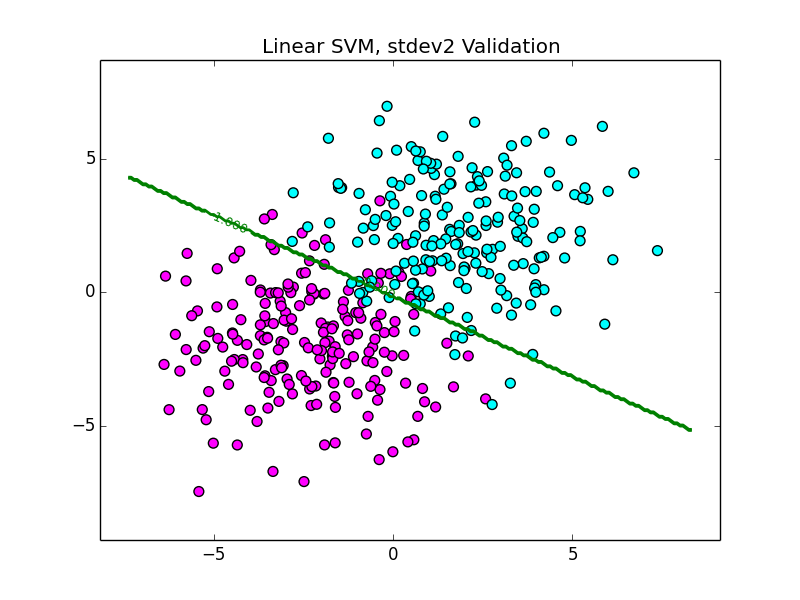
\includegraphics[width=1\linewidth, height=1in]{linear_svm_stdev2_validation.png}
		\caption*{stdev2 (Validation)}
	\end{minipage}
	\begin{minipage}[b]{.24\linewidth}
		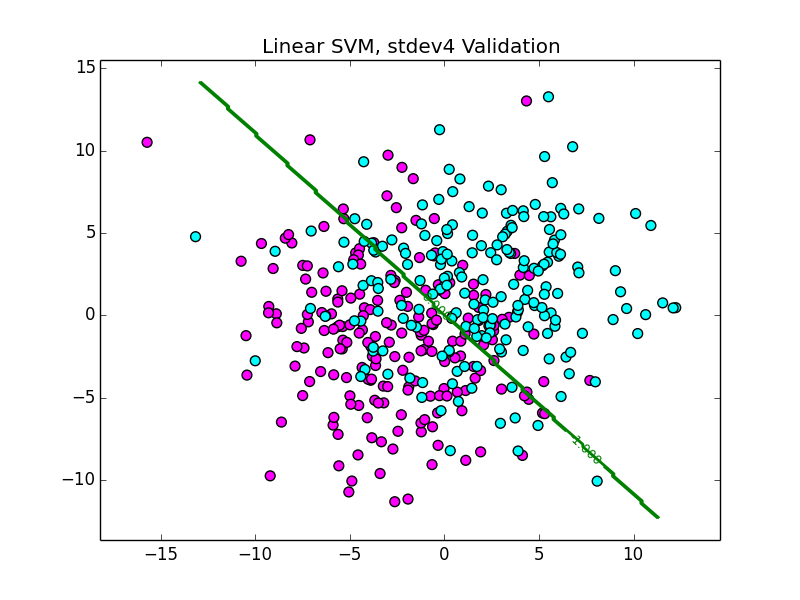
\includegraphics[width=1\linewidth, height=1in]{linear_svm_stdev4_validation.png}
		\caption*{stdev4 (Validation)}
	\end{minipage}
	\begin{minipage}[b]{.24\linewidth}
		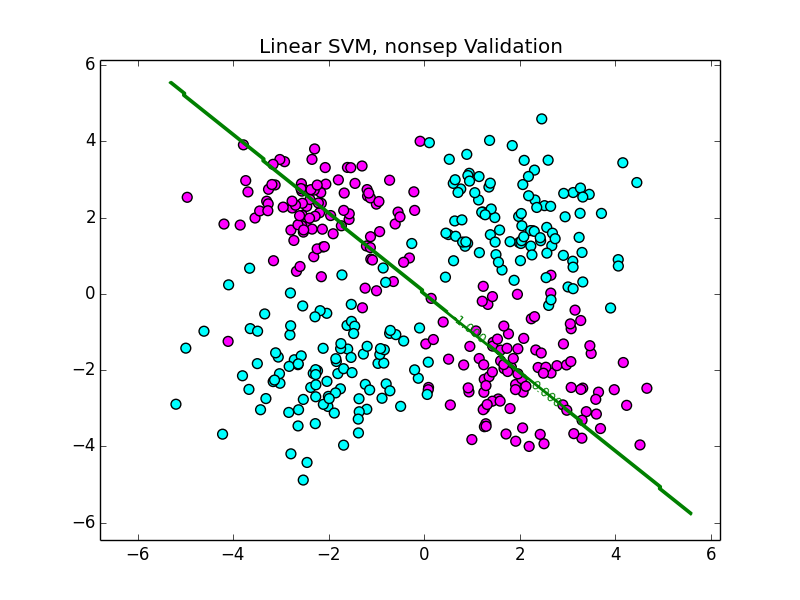
\includegraphics[width=1\linewidth, height=1in]{linear_svm_nonsep_validation.png}
		\caption*{nonsep (Validation)}
	\end{minipage}
	\caption{The decision boundaries generated by SVM plotted against the stdev1, stdev2, stdev4, and nonsep (training and validation) datasets}
\end{figure}

\begin{table}
\captionof{table}{Soft SVM Performance for Different Parameters and Kernels} 
\centering
\begin{tabular}{llllll}
\toprule
{} &                        Kernel &      $C$ &   $\sigma$ &    Number of Support Vectors & $1/||\mathbf{w}||$ \\
\midrule
&    Gaussian &    .01 &    .01 &   400 &    .0286 \\
&    Gaussian &    .01 &    .1 &   400 &    .0286 \\
&    Gaussian &    .01 &    1 &   400 &    .0286 \\
&    Gaussian &    .01 &    10 &   400 &    .0286 \\
&    Gaussian &    .01 &    100 &   400 &    .0286 \\
&    Gaussian &    .1 &    .01 &   400 &    .0141 \\
&    Gaussian &    .1 &    .1 &   400 &    .0141 \\
&    Gaussian &    .1 &    1 &   400 &    .0207 \\
&    Gaussian &    .1 &    10 &   400 &    .0141 \\
&    Gaussian &    .1 &    100 &   400 &    .0141 \\
&    Gaussian &    1 &    .01 &   400 &    .0017 \\
&    Gaussian &    1 &    .1 &   391 &    .0022 \\
&    Gaussian &    1 &    1 &   100 &    .0076 \\
&    Gaussian &    1 &    10 &   368 &    .0018 \\
&    Gaussian &    1 &    100 &   400 &    .0017 \\
&    Gaussian &    10 &    .01 &   400 &    .0017 \\
&    Gaussian &    10 &    .1 &   390 &    .0018 \\
&    Gaussian &    10 &    1 &   71 &    .0017 \\
&    Gaussian &    10 &    10 &   209 &    .0003 \\
&    Gaussian &    10 &    100 &   400 &    .0002 \\
&    Gaussian &    100 &    .01 &   400 &    .0017 \\
&    Gaussian &    100 &    .1 &   390 &    .0018 \\
&    Gaussian &    100 &    1 &   59 &    .0002 \\
&    Gaussian &    100 &    10 &   159 &    7.51e-5 \\
&    Gaussian &    100 &    100 &   399 &    1.77e-5 \\
&    Linear &    .01 &    N/A &   399 &    .0282 \\
&    Linear &    .1 &    N/A &   393 &    .0133 \\
&    Linear &    1 &    N/A &   392 &    .0017 \\
&    Linear &    10 &    N/A &   393 &    .0002 \\
&    Linear &    100 &    N/A &   397 &    1.8e-5 \\
\midrule
\bottomrule
\end{tabular}
\end{table}



\end{document}
Status API Training Shop Blog About Pricing
© 2015 GitHub, Inc. Terms Privacy Security Contact Help